\documentclass[tikz,border=4pt]{standalone}
\usetikzlibrary{arrows.meta,positioning,fit,backgrounds}

\definecolor{garnet}{HTML}{73000A}
\definecolor{black90}{HTML}{363636}
\definecolor{neutral10}{HTML}{ECECEC}
\definecolor{sandstorm}{HTML}{FFF2E3}
\definecolor{rose}{HTML}{CC2E40}
\definecolor{atlantic}{HTML}{466A9F}
\definecolor{congaree}{HTML}{1F414D}
\definecolor{horseshoe}{HTML}{65780B}

\begin{document}
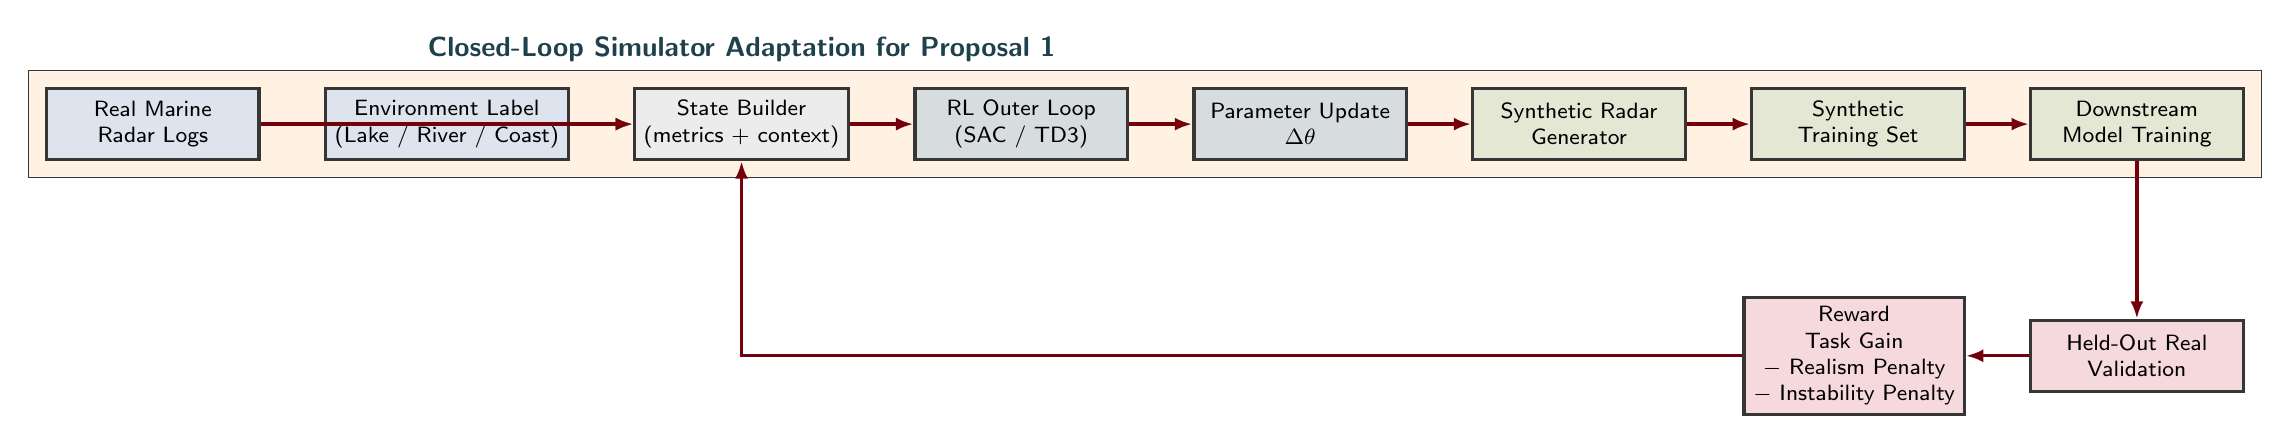
\begin{tikzpicture}[
  font=\sffamily\footnotesize,
  node distance=8mm and 8mm,
  block/.style={draw=black90, minimum height=9mm, minimum width=27mm, align=center, very thick},
  flow/.style={-{Latex[length=2.2mm]}, very thick, draw=garnet},
]

\node[block, fill=atlantic!18] (real) {Real Marine\\Radar Logs};
\node[block, fill=atlantic!18, right=of real] (env) {Environment Label\\(Lake / River / Coast)};
\node[block, fill=neutral10, right=of env] (state) {State Builder\\(metrics + context)};
\node[block, fill=congaree!18, right=of state] (policy) {RL Outer Loop\\(SAC / TD3)};
\node[block, fill=congaree!18, right=of policy] (theta) {Parameter Update\\$\Delta\theta$};
\node[block, fill=horseshoe!18, right=of theta] (sim) {Synthetic Radar\\Generator};
\node[block, fill=horseshoe!18, right=of sim] (train) {Synthetic\\Training Set};
\node[block, fill=horseshoe!18, right=of train] (model) {Downstream\\Model Training};

\node[block, fill=rose!18, below=20mm of model] (val) {Held-Out Real\\Validation};
\node[block, fill=rose!18, left=of val] (reward) {Reward\\Task Gain\\$-$ Realism Penalty\\$-$ Instability Penalty};

\draw[flow] (real) -- (state);
\draw[flow] (env) -- (state);
\draw[flow] (state) -- (policy);
\draw[flow] (policy) -- (theta);
\draw[flow] (theta) -- (sim);
\draw[flow] (sim) -- (train);
\draw[flow] (train) -- (model);
\draw[flow] (model) -- (val);
\draw[flow] (val) -- (reward);
\draw[flow] (reward.west) -| ([yshift=-8mm]state.south) -- (state.south);

\begin{scope}[on background layer]
  \node[draw=black90, inner sep=6pt, fit=(real)(env)(state)(policy)(theta)(sim)(train)(model), fill=sandstorm] {};
\end{scope}

\node[font=\bfseries\sffamily, text=congaree, above=2mm of state.north] {Closed-Loop Simulator Adaptation for Proposal 1};
\end{tikzpicture}
\end{document}
